% LuaLaTeX

\documentclass[a4paper, twoside, 12pt]{article}
\usepackage[latin]{babel}
%\usepackage[landscape, left=3cm, right=1.5cm, top=2cm, bottom=1cm]{geometry} % okraje stranky
\usepackage[landscape, a4paper, mag=1080, truedimen, left=2cm, right=1.5cm, top=1.8cm, bottom=1cm]{geometry} % okraje stranky

\usepackage{fontspec}
\setmainfont[Ligatures={Common, TeX}]{Junicode}
%\setmainfont{Junicode}

% shortcut for Junicode without ligatures (for the Czech texts)
\newfontfamily\nlfont[Ligatures={Common, TeX}]{Junicode}

% Hebrew font: http://scripts.sil.org/cms/scripts/page.php?site_id=nrsi&id=SILHebrUnic2
\newfontfamily\hebfont[Scale=1]{Ezra SIL}

\usepackage{multicol}
\usepackage{color}
\usepackage{lettrine}
\usepackage{fancyhdr}

% usual packages loading:
\usepackage{luatextra}
\usepackage{graphicx} % support the \includegraphics command and options
\usepackage{gregoriotex} % for gregorio score inclusion
\usepackage{gregoriosyms}
\usepackage{wrapfig} % figures wrapped by the text
\usepackage{parcolumns}
\usepackage[contents={},opacity=1,scale=1,color=black]{background}
\usepackage{tikzpagenodes}
\usetikzlibrary{calc}

% Commands used to produce a typical "Conventus" booklet

\newenvironment{titulusOfficii}{\begin{center}}{\end{center}}
\newcommand{\dies}[1]{#1

}
\newcommand{\nomenFesti}[1]{\textbf{\Large #1}

}
\newcommand{\celebratio}[1]{#1

}

\newcommand{\hora}[1]{%
\vspace{0.5cm}{\large \textbf{#1}}

\fancyhead[LE]{\thepage\ / #1}
\fancyhead[RO]{#1 / \thepage}
\addcontentsline{toc}{subsection}{#1}
}

% larger unit than a hora
\newcommand{\divisio}[1]{%
\begin{center}
{\Large \textsc{#1}}
\end{center}
\fancyhead[CO,CE]{#1}
\addcontentsline{toc}{section}{#1}
}

% a part of a hora, larger than pars
\newcommand{\subhora}[1]{
\begin{center}
{\large \textit{#1}}
\end{center}
%\fancyhead[CO,CE]{#1}
\addcontentsline{toc}{subsubsection}{#1}
}

% rubricated inline text
\newcommand{\rubricatum}[1]{\textit{#1}}

% standalone rubric
\newcommand{\rubrica}[1]{\vspace{3mm}\rubricatum{#1}}

\newcommand{\notitia}[1]{\textcolor{red}{#1}}

\newcommand{\scriptura}[1]{\hfill \small\textit{#1}}

\newcommand{\translatioCantus}[1]{\vspace{1mm}%
{\noindent\footnotesize \nlfont{#1}}}

% pruznejsi varianta nasledujiciho - umoznuje nastavit sirku sloupce
% s prekladem
\newcommand{\psalmusEtTranslatioB}[3]{
  \vspace{0.5cm}
  \begin{parcolumns}[colwidths={2=#3}, nofirstindent=true]{2}
    \colchunk{
      \input{#1}
    }

    \colchunk{
      \vspace{-0.5cm}
      {\footnotesize \nlfont
        \input{#2}
      }
    }
  \end{parcolumns}
}

\newcommand{\psalmusEtTranslatio}[2]{
  \psalmusEtTranslatioB{#1}{#2}{8.5cm}
}


\newcommand{\canticumMagnificatEtTranslatio}[1]{
  \psalmusEtTranslatioB{#1}{temporalia/extra-adventum-vespers/magnificat-boh.tex}{12cm}
}
\newcommand{\canticumBenedictusEtTranslatio}[1]{
  \psalmusEtTranslatioB{#1}{temporalia/extra-adventum-laudes/benedictus-boh.tex}{10.5cm}
}

% volne misto nad antifonami, kam si zpevaci dokresli neumy
\newcommand{\hicSuntNeumae}{\vspace{0.5cm}}

% prepinani mista mezi notovymi osnovami: pro neumovane a neneumovane zpevy
\newcommand{\cantusCumNeumis}{
  \setgrefactor{17}
  \global\advance\grespaceabovelines by 5mm%
}
\newcommand{\cantusSineNeumas}{
  \setgrefactor{17}
  \global\advance\grespaceabovelines by -5mm%
}

% znaky k umisteni nad inicialu zpevu
\newcommand{\superInitialam}[1]{\gresetfirstlineaboveinitial{\small {\textbf{#1}}}{\small {\textbf{#1}}}}

% pars officii, i.e. "oratio", ...
\newcommand{\pars}[1]{\textbf{#1}}

\newenvironment{psalmus}{
  \setlength{\parindent}{0pt}
  \setlength{\parskip}{5pt}
}{
  \setlength{\parindent}{10pt}
  \setlength{\parskip}{10pt}
}

%%%% Prejmenovat na latinske:
\newcommand{\nadpisZalmu}[1]{
  \hspace{2cm}\textbf{#1}\vspace{2mm}%
  \nopagebreak%

}

% mode, score, translation
\newcommand{\antiphona}[3]{%
\hicSuntNeumae
\superInitialam{#1}
\includescore{#2}

#3
}
 % Often used macros
%%%% Preklady jednotlivych zpevu (nektere se opakuji, a je dobre mit je
% vsechny na jedne hromade)

\newcommand{\trOratioAnteOfficium}{\translatioCantus{Otevři, Pane, má ústa, abych chválil tvé svaté jméno.
Očisti mé srdce od všech marnivých, zvrácených a~jiných myšlenek, osvěť rozum, rozněť cit,
abych mohl důstojně, soustředěně a~zbožně recitovat a~vysloužil si být
vyslyšen před tváří tvé velebnosti. Skrze Krista…}}

\newcommand{\trOratioPostOfficium}{\translatioCantus{\textit{Následující modlitbu
opatřil pro ty, kdo ji zbožně vyřknou po hodinkách, zesnulý papež Lev X.
odpustky za hříchy vzniklé při konání hodinek z~lidské křehkosti. Říká se
vkleče.}
Svatosvaté a~nerozdílné Trojici, ukřižovanému lidství našeho Pána Ježíše
Krista, přeblažené a~přeslavné plodné neporušenosti vždy Panny Marie
i~souhrnu všech svatých buď ode všeho stvoření věčná chvála, čest a~sláva, nám
pak buď dáno odpuštění všech hříchů, po nekonečné věky věků. Amen.}}

% HOURS ---

\newcommand{\trAntI}{\translatioCantus{Jasné narození slavné Panny Marie,
z pokolení (dosl. ze semene) Abrahámova, vzešlé z kmene Judova, z rodu Davidova.}}
\newcommand{\trAntII}{\translatioCantus{Dnes je Narození svaté Panny 
Marie, jejíž předrahý život osvěcuje všechny církve.}}

\newcommand{\trAntIII}{\translatioCantus{Maria, jež vzešla 
z královského rodu, září; myslí i duchem ji zbožně prosíme, aby 
nám pomáhala svými přímluvami.}}

\newcommand{\trAntIV}{\translatioCantus{Srdcem i duchem pějme Kristu 
k slávě o této svaté slavnosti vznešené Rodičky Boží Marie.}}

\newcommand{\trAntV}{\translatioCantus{Příjemně \notitia{?} 
oslavujme Narození blahoslavené Marie,
aby se ona za nás přimlouvala u Pána Ježíše Krista.}}

\newcommand{\trCapituli}{\translatioCantus{Před věky, na počátku mě stvořil, potrvám věčně. Ve svatém Stanu jsem před ním konala službu.}}

\newcommand{\trRespVesp}{\translatioCantus{Buď zdráva, Maria,
plná milosti: \grestar{} Pán s tebou. \Vbardot{} Požehnaná jsi mezi ženami,
a požehnaný plod života (ve smyslu lůna, břicha) tvého.}}

\newcommand{\trVersus}{\translatioCantus{\Vbardot{} Dnes je Narození svaté Panny Marie. \Rbardot{} Jejíž předrahý život osvěcuje všechny církve.}}

\newcommand{\trAntMagnificatI}{\translatioCantus{Konejme památku
veledůstojného narození slavné Panny Marie,
jíž se dostalo mateřské důstojnosti bez ztráty panenské cudnosti.}}

% Tento preklad je vice nez nejisty a ani alternativy, ktere jsem
% videl, me nepresvedcily...
\newcommand{\trAntBenedictus}{\translatioCantus{Slavnostně slavme 
dnešní narození Marie, vždy Panny a Rodičky Boží: v něm se objevuje
vysokost trůnu (totiž Marie, trůnu Božího Syna), aleluja.}}

\newcommand{\trAntMagnificatII}{\translatioCantus{Tvé narození,
Bohorodičko Panno, vyhlásilo radost celému světu:
z tebe totiž vzešlo Slunce spravedlnosti, Kristus, náš Bůh:
jenž zrušil kletbu a dal nám požehnání: přemohl smrt a dal nám život věčný.}}

\newcommand{\trOrationis}{\translatioCantus{Prosíme tě, Bože, 
uděl svým služebníkům dar nebeské milosti,
aby těm, jimž slehnutím blahoslavené Panny vyvstal počátek spásy, 
slavnost k poctě jejího narození přinesla
rozhojnění pokoje.
Skrze tvého Syna, našeho Pána Ježíše Krista, který s tebou žije a kraluje,
Bůh, v jednotě Ducha svatého po všechny věky věků.}}

\newcommand{\trFideliumAnimae}{\translatioCantus{\Vbardot{} Duše věrných ať pro
milosrdenství Boží odpočívají v~pokoji. \Rbardot{} Amen.}}

% Completorium

\newcommand{\trJubeDomne}{\translatioCantus{Rač, pane, požehnat.}}

\newcommand{\trComplBenedictio}{\translatioCantus{Pokojnou noc a~svatou smrt
nechť nám dopřeje všemohoucí Pán. \Rbardot{} Amen.}}

\newcommand{\trComplLectioBr}{\translatioCantus{Buďte střízliví, bděte.
Váš protivník Ďábel obchází jako lev řvoucí a~hledá, koho by pohltil.
Postavte se proti němu pevní ve víře.  Ale ty, Pane, smiluj se nad námi.
\Rbardot{} Bohu díky.}}

\newcommand{\trComplAntI}{\translatioCantus{Rač se smilovati nade mnou,
Hospodine, a vyslyš mou modlitbu.}}

\newcommand{\trComplCapituli}{\translatioCantus{Jsi přece, Hospodine,
uprostřed nás a~jmenujeme se po tobě.  Neopouštěj nás, Pane, náš Bože.}}

\newcommand{\trRespCompl}{\translatioCantus{Do tvých rukou, Pane, \grestar{}
poroučím svého ducha. \Vbardot{} Ty mne zachráníš, Pane, Bože věrný.}}

\newcommand{\trComplVersus}{\translatioCantus{\Vbardot{} Střez mne jako zřítelnici oka,
aleluja. \Rbardot{} Ve stínu svých křídel uschovej mne, aleluja.}}

\newcommand{\trAntSalvaNos}{\translatioCantus{Ochraňuj nás, Pane, když
bdíme, a~buď s~námi, když spíme, ať bdíme s~Kristem a~odpočíváme v~pokoji.}}

\newcommand{\trComplOrationis}{\translatioCantus{Zavítej, prosíme, Pane, sem
do našeho příbytku a~daleko od něj zažeň všechny úklady nepřítele. Ať tu
bydlí tví svatí andělé a~tvoje požehnání buď nad ním stále. Skrze…}}

\newcommand{\trSalveRegina}{\translatioCantus{Zdrávas Královno, matko
milosrdenství, živote, sladkosti a naděje naše, buď zdráva!
K tobě voláme, vyhnaní synové Evy,
k tobě vzdycháme, lkajíce a plačíce
v tomto slzavém údolí.
A proto, orodovnice naše,
obrať k nám své milosrdné oči
a Ježíše, požehnaný plod života svého,
nám po tomto putování ukaž,
ó milostivá, ó přívětivá,
ó přesladká, Panno Maria!}}

\newcommand{\trOraProNobis}{\translatioCantus{\Vbardot{} 
Oroduj za nás, svatá Boží Rodičko,
\Rbardot{} aby nám Kristus dal účast na svých zaslíbeních.}}

% Matutinum

\newcommand{\trMatInvitatorium}{\translatioCantus{}}

\newcommand{\trMatVeniteA}{\translatioCantus{Pojďte, chvalme s~radostí Pána,
s~jásotem slavme Boha, svou spásu; předstupme před tvář jeho s~díky, písně plesu pějme jemu.}}

\newcommand{\trMatVeniteB}{\translatioCantus{Neboť Bůh veliký jest Hospodin, a~král nade všecky bohy.
Jsouť v~jeho ruce všecky hlubiny země, temena hor jsou majetek jeho.}}

\newcommand{\trMatVeniteC}{\translatioCantus{Jehoť jest moře, neb on je učinil; i~souš
je dílo jeho rukou. Pojďme, klanějme se, padněme, klekněme před Pánem, svým
tvůrcem. Jeť on Pán, náš Bůh, a~my jsme lid, jejž on vodí a~ovce, jež pase.}}

\newcommand{\trMatVeniteD}{\translatioCantus{Kéž byste poslechli dnes hlasu jeho:
,,Nezatvrzujte svých srdcí jak v~Hádce, jak v~Pokušení na poušti, kde vaši otcové pokoušeli mne,
zkoušeli mne, ač vídali skutky mé.``}}

\newcommand{\trMatVeniteE}{\translatioCantus{Čtyřicet roků mrzel jsem se na to pokolení
a~řekl jsem: ,,Lid je to myslí stále bloudící``! Oni však nechtěli znáti mé cesty, takže jsem
přisáhl ve svém hněvu: ,,Nedojdou odpočinku mého!\mbox{}``}}

\newcommand{\trMatAntI}{\translatioCantus{}}

\newcommand{\trMatAntII}{\translatioCantus{}}

\newcommand{\trMatAntIII}{\translatioCantus{}}

\newcommand{\trMatVersusI}{\translatioCantus{}}

\newcommand{\trMatAbsolutioI}{\translatioCantus{Vyslyš Pane Ježíši Kriste
prosby svých služebníků \gredagger{} a~smiluj se nad námi, \grestar{} jenž
s~Otcem a~Duchem…}}

\newcommand{\trMatBenedictioI}{\translatioCantus{Rač, pane, požehnat.
Věčný Otec nám stále žehnej. \Rbardot{} Amen.}}

\newcommand{\trMatLecI}{\translatioCantus{Kéž by mě zulíbal polibky svých úst. 
Tvé milování je nad víno lahodnější;
vybraně voní tvé voňavky;
rozlévající se olej je tvé jméno,
proto tě dívky milují.
Strhni mě za sebou, poběžme!
Král mě uvedl do svých komnat;
budeš nám radostí a jásotem.
Víc než víno oslavíme tvé milování;
věru po právu jsi milován!
Snědá jsem, a přece krásná, jeruzalémské dcery,
jako stany kedarské,
jako šalmské závěsy.
}}

\newcommand{\trMatRespI}{\translatioCantus{}}

\newcommand{\trMatBenedictioII}{\translatioCantus{Rač, pane, požehnat.
Jednorozený Boží Syn nám žehnej \grestar{} a nám pomáhej. \Rbardot{} Amen.}}

\newcommand{\trMatLecII}{\translatioCantus{Nehleďte na mou osmahlou pleť:
to mě slunce ožehlo.
Synové mé matky se na mne rozzlobili,
poslali mě hlídat vinice.
A svou vinici, tu jsem nehlídala!
Pověz mi tedy, ty, jehož miluje mé srdce:
kam zavedeš své stádo pást,
kde ho necháš za poledne odpočívat?
Abych už nebloudila jako tulačka
poblíž stád druhů tvých.
Nevíš-li to, nejrásnější z žen,
jdi po stopách stáda
a kůzlata svá zaveď, ať se pasou
poblíž obydlí pastýřů.
Ke své klisně zapřažené do vozu faraonova
tebe, mé milá, přirovnávám.
Stále krásné jsou tvé líce s náušnicemi
i tvé hrdlo v náhrdelnících.}}

\newcommand{\trMatRespII}{\translatioCantus{}}

\newcommand{\trMatBenedictioIII}{\translatioCantus{Rač, pane, požehnat.
Milost Ducha Svatého ať osvítí nám smysly \grestar{} i srdce. \Rbardot{} Amen.}}

\newcommand{\trMatLecIII}{\translatioCantus{Zhotovíme ti zlaté náušnice
a kuličky ze stříbra.
Když král stoluje,
vydechuje můj nard svou vůni.
Můj milý je polštářek s myrhou,
jenž mi odpočívá mezi ňadry.
Můj milý je hrozen šáchoru
ve vinicích v Engadi.
Jak jsi krásná, milá moje,
jak jsi krásná!
Tvé oči jsou holubice.
Jak jsi krásný, můj milý,
jak líbezný!
Naše lože je samá zeleň.
Trámoví našeho domu je z cedru,
naše ostění z cypřiše.}}

\newcommand{\trMatRespIII}{\translatioCantus{}}

\newcommand{\trMatAntIV}{\translatioCantus{}}

\newcommand{\trMatAntV}{\translatioCantus{}}

\newcommand{\trMatAntVI}{\translatioCantus{}}

\newcommand{\trMatVersusII}{\translatioCantus{}}

\newcommand{\trMatAbsolutioII}{\translatioCantus{
Tvá milost a laskavost nechť nám pomáhá, jenž žiješ a vládneš s Otcem a Svatým Duchem na věky věků.}}

\newcommand{\trMatBenedictioIV}{\translatioCantus{Rač, pane, požehnat.
Bůh Otec všemohoucí, \grestar{} buď k nám milostivý a odpouštějící. \Rbardot{} Amen.}}

\newcommand{\trMatLecIV}{\translatioCantus{}}

\newcommand{\trMatRespIV}{\translatioCantus{}}

\newcommand{\trMatBenedictioV}{\translatioCantus{}}

\newcommand{\trMatLecV}{\translatioCantus{}}

\newcommand{\trMatRespV}{\translatioCantus{}}

\newcommand{\trMatBenedictioVI}{\translatioCantus{Rač, pane, požehnat.
Bůh rozněť v nás oheň své lásky. \Rbardot{} Amen.}}

\newcommand{\trMatLecVI}{\translatioCantus{}}

\newcommand{\trMatRespVI}{\translatioCantus{}}

\newcommand{\trMatAntVII}{\translatioCantus{}}

\newcommand{\trMatAntVIII}{\translatioCantus{}}

\newcommand{\trMatAntIX}{\translatioCantus{}}

\newcommand{\trMatVersusIII}{\translatioCantus{}}

\newcommand{\trMatAbsolutioIII}{\translatioCantus{Z okovů našich hříchů,
\grestar{} vysvoboď nás všemohoucí a milosrdný Pán. \Rbardot{} Amen.}}

\newcommand{\trMatBenedictioVII}{\translatioCantus{Rač, pane, požehnat.
Čtení evangelia nechť je nám \grestar{} spásou a ochranou. \Rbardot{} Amen.}}

\newcommand{\trMatLecVIIa}{\translatioCantus{
  Rodokmen Ježíše Krista, syna Davidova, syna Abrahámova:
  Abrahám zplodil Izáka,
  Izák zplodil Jakuba.}}

\newcommand{\trMatLecVIIb}{\translatioCantus{}}

\newcommand{\trMatRespVII}{\translatioCantus{}}

\newcommand{\trMatBenedictioVIII}{\translatioCantus{Rač, pane, požehnat.
\Rbardot{} Amen.}}

\newcommand{\trMatLecVIII}{\translatioCantus{}}

\newcommand{\trMatRespVIII}{\translatioCantus{}}

\newcommand{\trMatBenedictioIX}{\translatioCantus{Rač, pane, požehnat.
Do společnosti občanů nebes \grestar{} ať nás dovede král andělů.
\Rbardot{} Amen.}}

\newcommand{\trMatLecIX}{\translatioCantus{}}

% from the Czech Liturgia horarum
\newcommand{\trTeDeum}{\begin{translatioMulticol}{3}

Bože, tebe chválíme, 
tebe, Pane, velebíme.

Tebe, věčný Otče, 
oslavuje celá země.

Všichni andělé, 
cherubové i~serafové,

všechny mocné nebeské zástupy 
bez ustání volají:

Svatý, Svatý, Svatý, 
Pán, Bůh zástupů.

Plná jsou nebesa i~země 
tvé vznešené slávy.

Oslavuje tě 
sbor tvých apoštolů,

chválí tě 
velký počet proroků,

vydává o~tobě svědectví 
zástup mučedníků;

a~po celém světě 
vyznává tě tvá církev:

neskonale velebný, 
všemohoucí Otče,

úctyhodný Synu Boží, 
pravý a~jediný,

božský Utěšiteli, 
Duchu svatý.

Kriste, Králi slávy, 
tys od věků Syn Boha Otce;

abys člověka vykoupil, 
stal ses člověkem a~narodil ses z~Panny;

zlomil jsi osten smrti 
a~otevřel věřícím nebe;

sedíš po Otcově pravici 
a~máš účast na jeho slávě.

Věříme, že přijdeš soudit, 

a~proto tě prosíme:
přispěj na pomoc svým služebníkům, 
vždyť jsi je vykoupil svou předrahou krví;

dej, ať se radují s~tvými svatými 
ve věčné slávě.

Zachraň, Pane, svůj lid, žehnej svému dědictví, 
veď ho a~stále pozvedej.

Každý den tě budeme velebit 
a~chválit tvé jméno po všechny věky.

Pomáhej nám i~dnes, 
ať se nedostaneme do područí hříchu.

Smiluj se nad námi, Pane, 
smiluj se nad námi.

Ať spočine na nás tvé milosrdenství, 
jak doufáme v~tebe.

Pane, k~tobě se utíkáme, 
ať nejsme zahanbeni na věky. 
\end{translatioMulticol}}

\newcommand{\trMatEvangelium}{\translatioCantus{
  Rodokmen Ježíše Krista, syna Davidova, syna Abrahámova:
  Abrahám zplodil Izáka,
  Izák zplodil Jakuba,
  Jakub zplodil Judu a jeho bratry,
  Juda zplodil Farese a Zaru z Tamary,
  Fares zplodil Esroma,
  Esrom zplodil Arama,
  Aram zplodil Aminadaba,
  Aminadab zplodil Naasona,
  Naason zplodil Salmona,
  Salmon zplodil Boaze z Rahaby,
  Boaz zplodil Jobeda z Rut,
  Jobed zplodil Jessea,
  Jesse zplodil krále Davida.
  David zplodil Šalomouna z Uriášovy ženy,
  Šalomoun zplodil Roboama,
  Roboam zplodil Abiu,
  Abia zplodil Asu,
  Asa zplodil Josafata,
  Josafat zplodil Jorama,
  Joram zplodil Oziáše,
  Oziáš zplodil Joatama,
  Joatam zplodil Achaze,
  Achaz zplodil Ezechiáše,
  Ezechiáš zplodil Manasesa,
  Manases zplodil Amona,
  Amon zplodil Josiáše,
  Josiáš zplodil Jechoniáše a jeho bratry;
  tehdy došlo k odvlečení do Babylonu.
  Po odvlečení do Babylonu:
  Jechoniáš zplodil Salatiela,
  Salatiel zplodil Zorobabela,
  Zorobabel zplodil Abiuda,
  Abiud zplodil Eljakima,
  Eljakim zplodil Azora,
  Ator zplodil Sadoka,
  Sadok zplodil Achima,
  Achim zplodil Eliuda,
  Eliud zplodil Eleazara,
  Eleatar zplodil Matana,
  Matan zplodil Jakuba,
  Jakub zplodil Josefa, manžela Marie,
  z níž se narodil Ježíš, který se nazývá Kristus.}}

\newcommand{\trTeDecetLaus}{\translatioCantus{Tobě chvála, Tobě zpěvy, Tobě
sláva, Bohu Otci i~Synu i~Svatému Duchu, na věky věků. \Rbardot{} Amen.}}

% MASS ---

\newcommand{\trIntroitus}{\translatioCantus{Radujme se všichni
v Pánu, slavíce svátek ke cti Panny Marie: z něj se radují andělé
a spoluchválí Božího Syna. \textit{\color{red}Žl.} Má ústa vydala dobré slovo,
přednáším svá díla králi.}}

\newcommand{\trGraduale}{\translatioCantus{Požehnaná a ctihodná jsi,
Panno Maria: nedotčená (co do panenství) jsi byla shledána matkou
Spasitele. \Vbardot{} Panno Boží Rodičko, ten, jehož nepojme ani celý svět,
se uzavřel do tvých útrob, když se stal člověkem.}}

\newcommand{\trAlleluia}{\translatioCantus{Aleluja. \Vbardot{} Skvělá slavnost
slavné Panny Marie, z pokolení (dosl. ze semene) Abrahámova, vzešlé z kmene 
Judova, z rodu Davidova.}}

\newcommand{\trOffertorium}{\translatioCantus{Blažená jsi, Panno Maria,
tys nosila Stvořitele všeho; porodila jsi toho, který tě utvořil,
a na věky zůstáváš Pannou.}}

\newcommand{\trCommunio}{\translatioCantus{Budou mě blahoslavit
všechna pokolení, protože mi učinil veliké věci ten, který je mocný.}}

% LITTLE HOURS ---

\newcommand{\trVersusTertia}{\translatioCantus{\Vbardot{} \Rbardot{}}}

\newcommand{\trCapituliEtSic}{\translatioCantus{
Tak jsem se usadila na Sionu a v milovaném městě jsem nalezla odpočinek,
v Jeruzalémě vykonávám svou moc.
Zakořenila jsem u lidu plného slývy, na panství Páně, v jeho dědictví.}}

\newcommand{\trVersusSexta}{\translatioCantus{\Vbardot{} \Rbardot{}}}

\newcommand{\trCapituliInPlateis}{\translatioCantus{
Na planině jako skořicovník a akant jsem vydávala vůni, jako vybraná myrha
jsem voněla.}}

\newcommand{\trVersusNona}{\translatioCantus{\Vbardot{} \Rbardot{}}}
 % Czech translations of the proper texts

\newcommand{\annusEditionis}{2014}

% From git gregorio
\def\greendofsyllable{%
  \ifnum\greblockcusto=1\relax %
     \grelocalrightbox{}%
  \fi %
  \grepenalty{\greendofsyllablepenalty }%
  \relax%
}

%%%% Vicekrat opakovane kousky

\newcommand{\versusRegesTharsis}{
  \pars{Versus.}

  % Versus. %%%
    \includescore{temporalia/versus-reges.tex}

    \noindent \trVersus
    \vfill
}

\newcommand{\anteOrationem}{
  \rubrica{Ante Orationem, cantatur a Superiore:}

  \pars{Supplicatio Litaniæ.}

  \includescore{temporalia/supplicatiolitaniae.tex}

  \pars{Oratio Dominica.}

  \includescore{temporalia/oratiodominica.tex}

  \rubrica{Deinde dicitur ab Hebdomadario:}

  \includescore{temporalia/dominusvobiscum-solemnis.tex}

  \rubrica{In choro monialium loco Dominus vobiscum dicitur:}

  \includescore{temporalia/domineexaudi.tex}
}

\newcommand{\tuAutem}{
  \hspace{0.5cm}
  Tu autem, Dómine, miserére nobis.
  \Rbardot{} Deo grátias.
}

\setlength{\columnsep}{30pt} % prostor mezi sloupci

%%%%%%%%%%%%%%%%%%%%%%%%%%%%%%%%%%%%%%%%%%%%%%%%%%%%%%%%%%%%%%%%%%%%%%%%%%%%%%%%%%%%%%%%%%%%%%%%%%%%%%%%%%%%%
\begin{document}

% Here we set the space around the initial.
% Please report to http://home.gna.org/gregorio/gregoriotex/details for more details and options
\setspaceafterinitial{2.2mm plus 0em minus 0em}
\setspacebeforeinitial{2.2mm plus 0em minus 0em}

% Here we set the initial font. Change 43 if you want a bigger initial.
% Emit the initials in red.
\def\greinitialformat#1{%
{\color{red}\fontsize{43}{43}\selectfont #1}%
}

\pagestyle{empty}

%%%% Titulni stranka
\begin{titulusOfficii}
\dies{Die 6. Januaris.}
\nomenFesti{In Epiphania Domini.}
\celebratio{Duplex 1. classis.} % puvodne "cum Octava." Oktavy byly ale zruseny
\end{titulusOfficii}

% graphic
\vspace{1.5cm}
\begin{center}
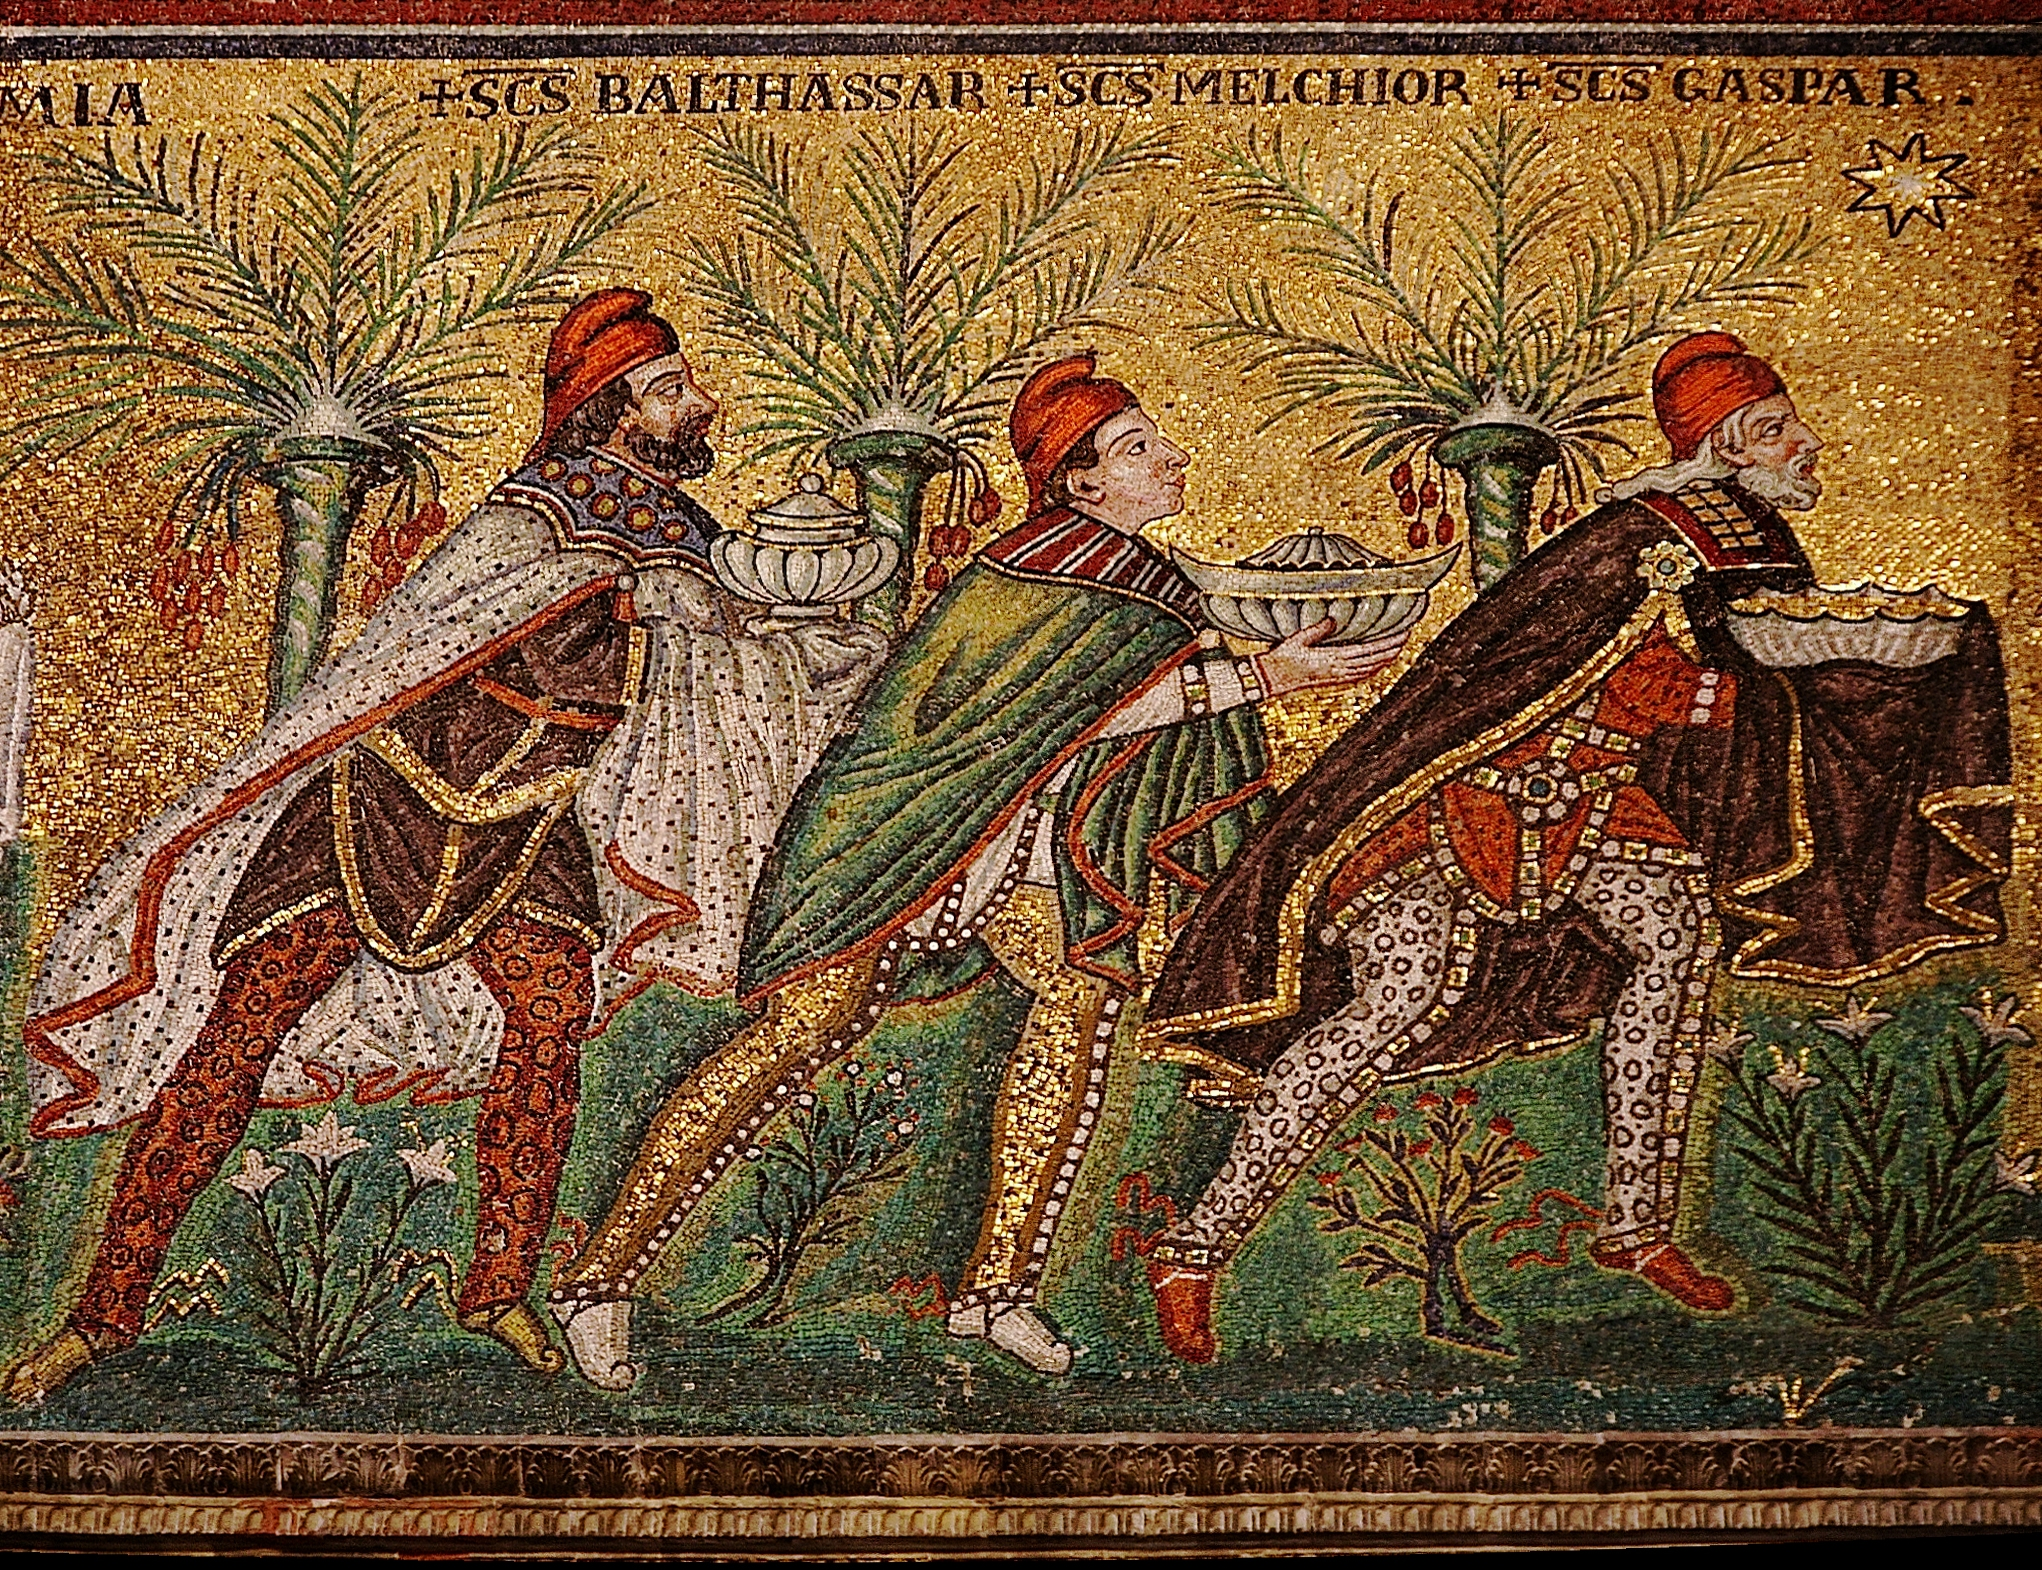
\includegraphics[width=10cm]{imagines/ravenna.jpg}
\end{center}

\vfill

\begin{center}
Ad usum et secundum consuetudines chori \guillemotright{}Conventus Choralis\guillemotleft.

Editio Sancti Wolfgangi \annusEditionis
\end{center}

\pagebreak

\renewcommand{\headrulewidth}{0pt} % no horiz. rule at the header
\fancyhf{}
\pagestyle{fancy}

\hora{In I. Vesperis.} %%%%%%%%%%%%%%%%%%%%%%%%%%%%%%%%%%%%%%%%%%%%%%%%%%%%%
\sideThumbs{I. Vesperis}

\label{deusinadiutorium}

\includescore{temporalia/deusinadiutorium-communis.tex}

\vfill

\pagebreak

\cantusCumNeumis

\pars{psalmus 1.}

\antiphona{II D}{temporalia/ant1.tex}

\trAntI

\scriptura{Psalmus 109.}

\includescore{temporalia/ps109-initium-ii-D-auto.tex}

%\translatioPsalmi{temporalia/ps109-boh.tex}
%\input{temporalia/ps109.tex}

\psalmusEtTranslatio{temporalia/ps109.tex}{temporalia/ps109-boh.tex}

\vfill

\pagebreak

\pars{psalmus 2.}

\antiphona{I g2}{temporalia/ant2.tex}

\trAntII

\scriptura{Psalmus 110.}

\includescore{temporalia/ps110-initium-i-g2-auto.tex}

% \translatioPsalmi{temporalia/ps110-boh.tex}
% \input{temporalia/ps110.tex}

\psalmusEtTranslatioB{temporalia/ps110.tex}{temporalia/ps110-boh.tex}{10cm}

\vfill

\pagebreak

\pars{psalmus 3.}

\antiphona{I g3}{temporalia/ant3.tex}

\trAntIII

\scriptura{Psalmus 111.}

\includescore{temporalia/ps111-initium-i-g3-auto.tex}

% \translatioPsalmi{temporalia/ps111-boh.tex}
% \input{temporalia/ps111.tex}

\psalmusEtTranslatio{temporalia/ps111.tex}{temporalia/ps111-boh.tex}

\vfill

\pagebreak

\pars{psalmus 4.}

\antiphona{IV E}{temporalia/ant4.tex}

\trAntIV

\scriptura{Psalmus 112.}

\includescore{temporalia/ps112-initium-iv-E-auto.tex}

%\translatioPsalmi{temporalia/ps112-boh.tex}
%\input{temporalia/ps112.tex}
\psalmusEtTranslatio{temporalia/ps112.tex}{temporalia/ps112-boh.tex}

\vfill

\pagebreak

\raggedcolumns

% Capitulum. %%%
\cantusSineNeumas

\label{capitulum}
\pars{Capitulum.} \scriptura{Isaiæ 60, 1}

\includescore{temporalia/capitulum-Surge.tex}

% preklad Jeruz. bible
\trCapituli

\vspace{1cm}
\pars{Responsorium breve.}

\superInitialam{VI.}
\includescore{temporalia/resp1v.tex}

\trRespVesp

\vfill

\pagebreak

% Hymnus. %%%
\pars{Hymnus.}

\superInitialam{III}
\includescore{temporalia/hym-HostisHerodes.tex}
\begin{translatioMulticol}{5}
Lorem ipsum dolor sit amet,\\
consectetur adipiscing elit,\\
sed do eiusmod tempor incididunt\\
ut labore et dolore magna aliqua.\columnbreak

Ut enim ad minim veniam,\\
quis nostrud exercitation\\
ullamco laboris nisi ut\\
aliquip ex ea commodo consequat.\columnbreak

Duis aute irure dolor\\
in reprehenderit in voluptate\\
velit esse cillum dolore eu\\
fugiat nulla pariatur.\columnbreak

Excepteur sint occaecat\\
cupidatat non proident,\\
sunt in culpa qui officia\\
deserunt mollit anim id est laborum.\columnbreak

Sláva tobě, Pane,\\
jenž ses dnes zjevil,\\
s Otcem i Svatým Duchem\\
na věčné věky.
Amen.
\end{translatioMulticol}


\versusRegesTharsis

\pagebreak

\cantusCumNeumis

\pars{Canticum B. Mariæ V.}\rubrica{ - in I. vesperis:}

\antiphona{VIII G2}{temporalia/ant-magn-vesp1.tex}

\trAntMagnificatI

\cantusSineNeumas
\includescore{temporalia/magnificat-initium-viii-G2.tex}

\psalmusEtTranslatioB{temporalia/magnificat.tex}{temporalia/magnificat-boh.tex}{10cm}

\pagebreak

\pars{Canticum B. Mariæ V.}\rubrica{ - in II. vesperis:}
\label{magnificatIIvesp}

\cantusCumNeumis

\antiphona{I D*}{temporalia/ant-magn-vesp2.tex}

\trAntMagnificatII

% antifona je dlouha a mista dost, dame Magnificat na novou stranku
\vfill
\pagebreak

\cantusSineNeumas
\includescore{temporalia/magnificat-initium-i-D_.tex}

% maly svindl, ale prizvukova struktura VIIIsoll-G2 a Isoll-D* je stejna
\psalmusEtTranslatio{temporalia/magnificat.tex}{temporalia/magnificat-boh.tex}

\pagebreak

\label{oratio}
\anteOrationem

\pagebreak

% Oratio. %%%
\pars{Oratio.}

\includescore{temporalia/oratio.tex}
\trOrationis

\vspace{1cm}
\rubrica{Hebdomadarius dicit iterum Dominus vobiscum. Postea cantatur a cantore:}
\vspace{2mm}

\includescore{temporalia/benedicamus-duplex-vesperae.tex}

\vfill

\pagebreak

\hora{Ad Completorium.} %%%%%%%%%%%%%%%%%%%%%%%%%%%%%%%%%%%%%%%%%%%%%%%%%%%%%%%%%%
\sideThumbs{{\scriptsize{}Completorium}}

\rubrica{Lector incipit:}

\includescore{temporalia/jubedomnebenedicere.tex}

\vfill

\pars{Benedictio.}

\includescore{temporalia/benedictio-noctemquietam.tex}

\vfill

\pars{Lectio brevis.}

\scriptura{1 Petr. 5, 8-9}

\includescore{temporalia/lectiobrevis-fratressobrii.tex}

\vfill

\pagebreak

\vspace{1cm}
\includescore{temporalia/deusinadiutorium-communis.tex}
\vspace{1cm}

\pars{psalmus 1.}

\scriptura{Psalmus 4.}

\includescore{temporalia/ps4-initium-dir-auto.tex}

%\translatioPsalmi{temporalia/ps4-boh.tex}
%\input{temporalia/ps4.tex}
\psalmusEtTranslatioB{temporalia/ps4.tex}{temporalia/ps4-boh.tex}{11.5cm}

\vfill

\pagebreak

\pars{psalmus 2.}

\scriptura{Psalmus 90.}

\includescore{temporalia/ps90-initium-dir-auto.tex}

%\translatioPsalmi{temporalia/ps90-boh.tex}
%\input{temporalia/ps90.tex}
\psalmusEtTranslatioB{temporalia/ps90.tex}{temporalia/ps90-boh.tex}{9.5cm}

\vfill

\pagebreak

\pars{psalmus 3.}

\scriptura{Psalmus 133.}

\includescore{temporalia/ps133-initium-dir-auto.tex}

%\translatioPsalmi{temporalia/ps133-boh.tex}
%\input{temporalia/ps133.tex}
\psalmusEtTranslatio{temporalia/ps133.tex}{temporalia/ps133-boh.tex}

\vfill

\pars{Hymnus}

\antiphona{VIII}{temporalia/hym-TeLucis.tex}

\vfill

\pagebreak

\hora{Ad Matutinum.} %%%%%%%%%%%%%%%%%%%%%%%%%%%%%%%%%%%%%%%%%%%%%%%%%%%%%%%%%%
\sideThumbs{Matutinum}

\subhora{In I. Nocturno}

\pars{psalmus 1.}

\scriptura{Psalmus 28, 1.2; \textbf{H72}}

\antiphona{VII a}{temporalia/matant1.tex}

\trMatAntI

\scriptura{Psalmus 28.}

\includescore{temporalia/ps28-initium-vii-a-auto.tex}

%\translatioPsalmi{temporalia/ps28-boh.tex}
%\input{temporalia/ps28.tex}
\psalmusEtTranslatioB{temporalia/ps28.tex}{temporalia/ps28-boh.tex}{10.5cm}

\vfill

\pagebreak

\pars{psalmus 2.}

\scriptura{Psalmus 45, 5; \textbf{H72}}

\antiphona{VI F}{temporalia/matant2.tex}

\trMatAntII

\scriptura{Psalmus 45.}

\includescore{temporalia/ps45-initium-vi-F-auto.tex}

%\translatioPsalmi{temporalia/ps45-boh.tex}
%\input{temporalia/ps45.tex}
\psalmusEtTranslatio{temporalia/ps45.tex}{temporalia/ps45-boh.tex}

\vfill

\pagebreak

\pars{psalmus 3.}

\scriptura{Psalmus 46, 7.8; \textbf{H72}}

\antiphona{I f}{temporalia/matant3.tex}

\trMatAntIII

\scriptura{Psalmus 46.}

\includescore{temporalia/ps46-initium-i-f-auto.tex}

%\translatioPsalmi{temporalia/ps46-boh.tex}
%\input{temporalia/ps46.tex}
\psalmusEtTranslatio{temporalia/ps46.tex}{temporalia/ps46-boh.tex}

\vfill

\pagebreak

\pars{Lectio I}
% De Isaia Prophéta.
\scriptura{Isaiæ 55, 1-4}

\textusEtTranslatio{
  Omnes sitiéntes, veníte ad aquas, et qui non habétis argéntum, properáte,
  émite, et comédite: veníte, émite absque argénto et absque ulla commutatióne
  vinum et lac.
  Quare appénditis argéntum non in pánibus, et labórem vestrum non in
  saturitáte? Audíte, audiéntes me, et comédite bonum, et delectábitur in
  crassitúdine ánima vestra.
  Inclináte aurem vestram, et veníte ad me; audíte, et vivet ánima vestra,
  et fériam vobíscum pactum sempitérnum, misericórdias David fidéles.
  Ecce testem pópulis dedi eum, ducem ac præceptórem géntibus.

  \tuAutem
}{\trMatLecI}{10cm}

\vfill

\responsorium{III}{temporalia/matresp1.tex}{\trMatRespI}

\vfill

\pagebreak

\pars{Lectio II}
\scriptura{Isaiæ 60, 1-6}

\textusEtTranslatio{
  Surge, illumináre, Jerúsalem, quia venit lumen tuum, et glória Dómini
  super te orta est.
  Quia ecce ténebræ opérient terram, et calígo pópulos; super te autem
  oriétur Dóminus, et glória ejus in te vidébitur.
  Et ambulábunt gentes in lúmine tuo, et reges in splendóre ortus tui.
  Leva in circúitu óculos tuos, et vide: omnes isti congregáti sunt,
  venérunt tibi; fílii tui de longe vénient et fíliæ tuæ de látere surgent.
  Tunc vidébis, et áfflues; mirábitur et dilatábitur cor tuum: quando
  convérsa fúerit ad te multitúdo maris; fortitúdo géntium vénerit tibi.
  Inundátio camelórum opériet te, dromedárii Mádian et Epha; omnes de Saba
  vénient, aurum et thus deferéntes, et laudem Dómino annuntiántes.

  \tuAutem
}{\trMatLecII}{10cm}

\vfill

\responsorium{II}{temporalia/matresp2.tex}{\trMatRespII}

\vfill

\pagebreak

\pars{Lectio III}
\scriptura{Isaiæ 61, 10-11; 62, 1}

\textusEtTranslatio{
  Gaudens gaudébo in Dómino, et exsultábit ánima mea in Deo meo, quia
  índuit me vestiméntis salútis, et induménto justítiæ circúmdedit me, quasi
  sponsum decorátum coróna, et quasi sponsam ornátam monílibus suis.
  Sicut enim terra profert germen suum, et sicut hortus semen suum
  gérminat, sic Dóminus Deus germinábit justítiam et laudem coram univérsis
  géntibus.
  Propter Sion non tacébo, et propter Jerúsalem non quiéscam, donec
  egrediátur ut splendor justus ejus, et salvátor ejus ut lampas accendátur.

  \tuAutem
}{\trMatLecIII}{10cm}

\vfill

\responsorium{II}{temporalia/matresp3.tex}{\trMatRespIII}

\vfill

\pagebreak

\subhora{In II. Nocturno}

\pars{psalmus 4.}

\scriptura{Psalmus 65, 4; \textbf{H73}}

\antiphona{IV E}{temporalia/matant4.tex}

\trMatAntIV

\scriptura{Psalmus 65.}

\includescore{temporalia/ps65-initium-iv-E-auto.tex}

%\translatioPsalmi{temporalia/ps65-boh.tex}
%\input{temporalia/ps65.tex}
\psalmusEtTranslatio{temporalia/ps65.tex}{temporalia/ps65-boh.tex}

\vfill

\pagebreak

\pars{psalmus 5.}

\scriptura{Psalmus 71, 10; \textbf{H73}}

\antiphona{I a2}{temporalia/matant5.tex}

\trMatAntV

\scriptura{Psalmus 71.}

\includescore{temporalia/ps71-initium-i-a2-auto.tex}

%\translatioPsalmi{temporalia/ps71-boh.tex}
%\input{temporalia/ps71.tex}
\psalmusEtTranslatio{temporalia/ps71.tex}{temporalia/ps71-boh.tex}

\vfill

\pagebreak

\pars{psalmus 6.}

\scriptura{Psalmus 85, 7.8; \textbf{H72}}

\antiphona{IV E}{temporalia/matant6.tex}

\trMatAntVI

\scriptura{Psalmus 85.}

\includescore{temporalia/ps85-initium-iv-E-auto.tex}

%\translatioPsalmi{temporalia/ps85-boh.tex}
%\input{temporalia/ps85.tex}
\psalmusEtTranslatio{temporalia/ps85.tex}{temporalia/ps85-boh.tex}

\vfill

\pagebreak

\pars{Lectio IV}
% Sermo sancti Leónis Papæ.
\scriptura{Sermo 2. de Epiphania.}

\textusEtTranslatio{
  Gaudéte in Dómino, dilectíssimi, íterum dico, gaudéte: quóniam brevi
  intervállo témporis, post solemnitátem Nativitátis Christi, festívitas
  declaratiónis ejus illúxit: et quem in illo die Virgo péperit, in hoc mundus
  agnóvit. Verbum enim caro factum, sic susceptiónis nostræ temperávit
  exórdia, ut natus Jesus et credéntibus maniféstus, et persequéntibus esset
  occúltus. Jam tunc ergo cæli enarravérunt glóriam Dei, et in omnem terram
  sonus veritátis exívit, quando et pastóribus exércitus Angelórum Salvatóris
  éditi annuntiátor appáruit, et Magos ad eum adorándum prǽvia stella
  perdúxit: ut a solis ortu usque ad occásum veri Regis generátio coruscáret,
  cum rerum fidem et regna Oriéntis per Magos díscerent, et Románum impérium
  non láteret.

  \tuAutem
}{\trMatLecIV}{10cm}

\vfill

\responsorium{V}{temporalia/matresp4.tex}{\trMatRespIV}

\vfill

\pagebreak

\pars{Lectio V}
\scriptura{Sermo 2. de Epiphania.}

\textusEtTranslatio{
  Nam et sævítia Heródis volens primórdia suspécti sibi Regis exstínguere,
  huic dispensatíoni nésciens serviébat: ut dum atróci inténtus facínori,
  ignótum sibi púerum indiscréta infántium cæde perséquitur, annuntiátum
  cǽlitus dominatóris ortum insígnior ubíque fama loquerétur: quam promptiórem
  ad narrándum, diligentiorémque faciébat et supérnæ significatiónis nóvitas,
  et cruentíssimi persecutóris impíetas. Tunc autem étiam Ægýpto Salvátor
  illátus est, ut gens antíquis erróribus dédita, jam ad vicínam salútem per
  occúltam grátiam signarétur: et quæ nondum ejécerat ab ánimo superstitiónem,
  jam hospítio recíperet veritátem.

  \tuAutem
}{\trMatLecV}{10cm}

\vfill

\responsorium{VII}{temporalia/matresp5.tex}{\trMatRespV}

\vfill

\pagebreak

\pars{Lectio VI}
\scriptura{Sermo 2. de Epiphania.}

\textusEtTranslatio{
  Agnoscámus ergo, dilectíssimi, in Magis adoratóribus Christi, vocatiónis
  nostræ fideíque primítias: et exsultántibus ánimis beátæ spei inítia
  celebrémus. Exínde enim in ætérnam hereditátem cœpimus introíre: exínde
  nobis Christum loquéntia Scripturárum arcána patuérunt, et véritas, quam
  Judæórum obcæcátio non récipit, ómnibus natiónibus lumen suum invéxit.
  Honorétur ítaque a nobis sacratíssimus dies, in quo salútis nostræ Auctor
  appáruit: et quem Magi infántem veneráti sunt in cunábulis, nos omnipoténtem
  adorémus in cælis. Ac sicut illi de thesáuris suis mýsticas Dómino múnerum
  spécies obtulérunt, ita et nos de córdibus nostris, quæ Deo sunt digna,
  promámus.

  \tuAutem
}{\trMatLecVI}{10cm}

\vfill

\responsorium{VIII}{temporalia/matresp6.tex}{\trMatRespVI}

\vfill

\pagebreak

\subhora{In III. Nocturno}

\pars{psalmus 7.}

\scriptura{Psalmus 94, 6.7; \textbf{H74}}

\antiphona{VIII G}{temporalia/matant7.tex}

\trMatAntVII

\scriptura{Psalmus 94.}

\includescore{temporalia/ps94-initium-viii-G.tex}

%\translatioPsalmi{temporalia/ps94-boh.tex}
%\begin{psalmus}
Præoccupémus fáciem ejus in confessi\textbf{ó}\-ne:~\grestar{}
et in psalmis jubi\emph{\-lé\-mus }\textbf{e}\-i. \Abardot{}

Quóniam Deus magnus \textbf{Dó}\-minus:~\grestar{}
et rex magnus super \emph{om\-nes }\textbf{de}\-os.

Quia in manu ejus sunt omnes fines \textbf{ter}\-ræ:~\grestar{}
et altitúdines mónti\emph{\-um i}\textbf{psí}\-us sunt. \Abardot{}

Quóniam ipsíus est mare, et ipse fecit \textbf{il}\-lud:~\grestar{}
et siccam manus ejus \emph{for\-ma}\textbf{vé}\-runt. \Abardot{}

Et nos pópulus páscuæ ejus, et oves manus \textbf{e}\-jus:~\grestar{}
Hódie si vocem ejus audiéritis, nolíte obduráre \emph{cor\-da }\textbf{ve}\-stra:

Sicut in irritatióne, secúndum diem tentatiónis in de\textbf{sé}\-rto:~\gredagger{}
ubi tentavérunt me patres \textbf{ve}\-stri,~\grestar{}
probavérunt me, et vidérunt ó\emph{\-pe\-ra }\textbf{me}\-a. \Abardot{}

Quadragínta annis offénsus fui generatióni \textbf{il}\-li,~\grestar{}
et dixi~: Semper hi \emph{er\-rant }\textbf{cor}\-de.

Et isti non cognovérunt vias meas, ut jurávi in ira \textbf{me}\-a:~\grestar{}
Si introíbunt in ré\emph{\-qui\-em }\textbf{me}\-am. \Abardot{}

Glória Pat\-ri et \textbf{Fí}\-lio,~\grestar{}
et Spirí\emph{\-tui }\textbf{San}\-cto.

Sicut erat in princípio, et nunc et \textbf{sem}\-per,~\grestar{}
et in sǽcula sæcu\emph{ló\-rum. }\textbf{A}\-men. \Abardot{}
\end{psalmus}

\psalmusEtTranslatioB{cantus/nrom02/ps94.tex}{temporalia/ps94-boh.tex}{9.5cm}

\vfill

\pagebreak

\pars{psalmus 8.}

\scriptura{Psalmus 95, 9; \textbf{H74}}

\antiphona{VI F}{temporalia/matant8.tex}

\trMatAntVIII

\scriptura{Psalmus 95.}

\includescore{temporalia/ps95-initium-vi-F-auto.tex}

%\translatioPsalmi{temporalia/ps95-boh.tex}
%\input{temporalia/ps95.tex}
\psalmusEtTranslatioB{temporalia/ps95.tex}{temporalia/ps95-boh.tex}{10cm}

\vfill

\pagebreak

\pars{psalmus 9.}

\scriptura{Psalmus 96, 7; \textbf{H74}}

\antiphona{VI F}{temporalia/matant9.tex}

\trMatAntIX

\scriptura{Psalmus 96.}

\includescore{temporalia/ps96-initium-vi-F-auto.tex}

%\translatioPsalmi{temporalia/ps96-boh.tex}
%\input{temporalia/ps96.tex}
\psalmusEtTranslatio{temporalia/ps96.tex}{temporalia/ps96-boh.tex}

\vfill

\pagebreak

\pars{Lectio VII}
% Léctio sancti Evangélii secúndum Matthǽum.
\scriptura{Matt 2, 1-12}

\textusEtTranslatio{
  Cum natus esset Jesus in Béthlehem Juda in diébus Heródis regis, ecce Magi
  ab Oriénte venérunt Jerosólymam, dicéntes: Ubi est qui natus est Rex
  Judæórum? Et réliqua.
}{\trMatLecVIIa}{10cm}

% Homilía sancti Gregórii Papæ.
\scriptura{Homilia 10. in Evang.}

\textusEtTranslatio{
  Sicut in lectióne evangélica, fratres caríssimi, audístis, cæli Rege nato,
  rex terræ turbátus est: quia nimírum terréna altitúdo confúnditur, cum
  celsitúdo cæléstis aperítur. Sed quæréndum nobis est, quidnam sit, quod,
  Redemptóre nato, pastóribus in Judǽa Angelus appáruit, atque ad adorándum
  hunc ab Oriénte Magos non Angelus, sed stella perdúxit? Quia vidélicet
  Judǽis, tamquam ratióne uténtibus, rationále ánimal, id est, Angelus
  prædicáre débuit: Gentíles vero, quia uti ratióne nesciébant, ad
  cognoscéndum Dóminum non per vocem, sed per signa perducúntur. Unde étiam
  per Paulum dícitur: Prophetíæ fidélibus datæ sunt, non infidélibus: signa
  autem infidélibus, non fidélibus. Quia et illis prophetíæ tamquam fidélibus,
  non infidélibus: et istis signa tamquam infidélibus, non fidélibus data
  sunt.

  \tuAutem
}{\trMatLecVIIb}{10cm}

\vfill

\responsorium{VIII}{temporalia/matresp7.tex}{\trMatRespVII}

\vfill

\pagebreak

\pars{Lectio VIII}
\scriptura{Homilia 10. in Evang.}

\textusEtTranslatio{
  Et notándum, quod Redemptórem nostrum, cum jam perféctæ esset ætátis, eísdem
  Gentílibus Apóstoli prǽdicant, eúmque párvulum, et necdum per humáni
  córporis offícium loquéntem, stella Géntibus denúntiat: quia nimírum
  ratiónis ordo poscébat, ut et loquéntem jam Dóminum loquéntes nobis
  prædicatóres innotéscerent, et necdum loquéntem eleménta muta prædicárent.
  Sed in ómnibus signis, quæ vel nascénte Dómino, vel moriénte eo monstráta
  sunt, considerándum nobis est, quanta fúerit in quorúmdam Judæórum corde
  durítia, qui hunc nec per prophetíæ donum, nec per mirácula agnovérunt.

  \tuAutem
}{\trMatLecVIII}{10cm}

\vfill

\responsorium{IV}{temporalia/matresp8.tex}{\trMatRespVIII}

\vfill

\pagebreak

\pars{Lectio IX}
\scriptura{Homilia 10. in Evang.}

\textusEtTranslatio{
  Omnia quippe eleménta auctórem suum venísse testáta sunt. Ut enim de eis
  quiddam usu humáno loquar: Deum hunc cæli esse cognovérunt, quia prótinus
  stellam misérunt. Mare cognóvit, quia sub plantis ejus se calcábile prǽbuit.
  Terra cognóvit, quia eo moriénte contrémuit. Sol cognóvit, quia lucis suæ
  rádios abscóndit. Saxa et paríetes cognovérunt, quia témpore mortis ejus
  scissa sunt. Inférnus agnóvit, quia hos, quos tenébat mórtuos, réddidit. Et
  tamen hunc, quem Dóminum ómnia insensibília eleménta sensérunt, adhuc
  infidélium Judæórum corda Deum esse mínime cognóscunt, et durióra saxis,
  scindi ad pœniténdum nolunt.

  \tuAutem
}{\trMatLecIX}{10cm}

\vfill

\pagebreak

% Te Deum

\pars{Hymnus Ambrosianus}

\superInitialam{III}
\includescore{temporalia/tedeum-solemnis.tex}

\trTeDeum

\vfill

\pagebreak

\hora{Ad Laudes.} %%%%%%%%%%%%%%%%%%%%%%%%%%%%%%%%%%%%%%%%%%%%%%%%%%%%%%%%%%
\sideThumbs{Laudes}

% Psalmi festivi (AM33, pg. 721):
% 66 // 92, 99, 62, Dan3, 148+149+150

\vspace{1cm}
\includescore{temporalia/deusinadiutorium-communis.tex}
\vspace{1cm}

\cantusSineNeumas

\pars{psalmus 1.}

\scriptura{Psalmus 66.}

\includescore{temporalia/ps66-initium-dir-auto.tex}

%\translatioPsalmi{temporalia/ps66-boh.tex}
%\input{temporalia/ps66.tex}
\psalmusEtTranslatio{temporalia/ps66.tex}{temporalia/ps66-boh.tex}

\vfill

\pagebreak

\pars{psalmus 2.}

\antiphona{II D}{temporalia/ant1.tex}

\trAntI

\scriptura{Psalmus 92.}

\includescore{temporalia/ps92-initium-ii-D-auto.tex}

%\translatioPsalmi{temporalia/ps92-boh.tex}
%\input{temporalia/ps92.tex}
\psalmusEtTranslatio{temporalia/ps92.tex}{temporalia/ps92-boh.tex}

\vfill

\pagebreak

\pars{psalmus 3.}

\antiphona{I g2}{temporalia/ant2.tex}

\trAntII

\scriptura{Psalmus 99.}

\includescore{temporalia/ps99-initium-i-g2-auto.tex}

%\translatioPsalmi{temporalia/ps99-boh.tex}
%\input{temporalia/ps99.tex}
\psalmusEtTranslatio{temporalia/ps99.tex}{temporalia/ps99-boh.tex}

\vfill

\pagebreak

\pars{psalmus 4.}

\antiphona{I g3}{temporalia/ant3.tex}

\trAntIII

\scriptura{Psalmus 62.}

\includescore{temporalia/ps62-initium-i-g3-auto.tex}

%\translatioPsalmi{temporalia/ps62-boh.tex}
%\input{temporalia/ps62.tex}
\psalmusEtTranslatio{temporalia/ps62.tex}{temporalia/ps62-boh.tex}

\vfill

\pagebreak

\pars{psalmus 5.}

\antiphona{IV E}{temporalia/ant4.tex}

\trAntIV

\scriptura{Canticum trium puerorum, Dan. 3, 57-88 et 56.}

\includescore{temporalia/dan3-initium-iv-E-auto.tex}

\psalmusEtTranslatioB{temporalia/dan3.tex}{temporalia/dan3-boh.tex}{10cm} % Canticum trium

\rubrica{Hic non dicitur Gloria Patri, neque Amen.}
\vspace{1cm}

\hicSuntNeumae
\includescore{temporalia/ant4.tex} % repeat the antiphon - new page

\vfill

\pagebreak

\pars{psalmus 6.}

\antiphona{VII c2}{temporalia/ant5.tex}

\trAntV

%
\scriptura{Psalmus 148.}

\includescore{temporalia/ps148-initium-vii-c2-auto.tex}

\newlength{\psVItransW}
\setlength{\psVItransW}{10.5cm}

%\translatioPsalmi{temporalia/ps148-boh.tex}
%\input{temporalia/ps148.tex}
\psalmusEtTranslatioB{temporalia/ps148.tex}{temporalia/ps148-boh.tex}{\psVItransW}

\rubrica{Hic non dicitur Gloria Patri.}

%
\scriptura{Psalmus 149.}

\includescore{temporalia/ps149-initium-vii-c2-auto.tex}

%\translatioPsalmi{temporalia/ps149-boh.tex}
%\input{temporalia/ps149.tex}
\psalmusEtTranslatioB{temporalia/ps149.tex}{temporalia/ps149-boh.tex}{\psVItransW}

\rubrica{Hic non dicitur Gloria Patri.}

%
\scriptura{Psalmus 150.}

\includescore{temporalia/ps150-initium-vii-c2-auto.tex}

%\translatioPsalmi{temporalia/ps150-boh.tex}
%\input{temporalia/ps150.tex}
\psalmusEtTranslatioB{temporalia/ps150.tex}{temporalia/ps150-boh.tex}{\psVItransW}

\pagebreak

\cantusSineNeumas

\pars{Capitulum.} \scriptura{Isaiæ 60, 1}

\includescore{temporalia/capitulum-Surge.tex}

% preklad Jeruz. bible
\trCapituli

\vspace{1cm}
\pars{Responsorium breve.}

\superInitialam{VI.}
\includescore{temporalia/respl.tex}

\trRespLaudes
\vfill

\pagebreak

\pars{Hymnus.}

\includescore{temporalia/hym-OSolaMagnarum.tex}
%BETHLEHEM! of noblest cities
%none can once with thee compare;
%thou alone the Lord from heaven
%didst for us Incarnate bear.
%
%Fairer than the sun at morning
%was the star that told His birth;
%to the lands their God announcing,
%hid beneath a form of earth.
%
%By its lambent beauty guided,
%see the eastern kings appear;
%see them bend, their gifts to offer-
%gifts of incense, gold, and myrrh.
%
%Solem things of mystic meaning!-
%Incense doth the God disclose;
%Gold a royal Child proclaimeth;
%Myrrh a future tomb foreshows.

\begin{translatioMulticol}{5}
Lorem ipsum dolor sit amet,\\
consectetur adipiscing elit,\\
sed do eiusmod tempor incididunt\\
ut labore et dolore magna aliqua.\columnbreak

Ut enim ad minim veniam,\\
quis nostrud exercitation\\
ullamco laboris nisi ut\\
aliquip ex ea commodo consequat.\columnbreak

Duis aute irure dolor\\
in reprehenderit in voluptate\\
velit esse cillum dolore eu\\
fugiat nulla pariatur.\columnbreak

Excepteur sint occaecat\\
cupidatat non proident,\\
sunt in culpa qui officia\\
deserunt mollit anim id est laborum.\columnbreak

Sláva tobě, Pane,\\
jenž ses dnes zjevil,\\
s Otcem i Svatým Duchem\\
na věčné věky.
Amen.
\end{translatioMulticol}


\vspace{0.5cm}

\versusRegesTharsis

\vfill

\pagebreak

\cantusCumNeumis

\pars{Canticum Zachariæ.}

\antiphona{VIII G2}{temporalia/ant-ben-laud.tex}

\trAntBenedictus

\includescore{temporalia/benedictus-initium-viiisoll-G2-auto.tex}

\psalmusEtTranslatioB{temporalia/benedictus.tex}{temporalia/benedictus-boh.tex}{10.5cm}

\vspace{0.5cm}

\vfill

\pagebreak

\cantusSineNeumas

\label{oratio}
\anteOrationem

\pagebreak

% Oratio. %%%
\pars{Oratio.}

\includescore{temporalia/oratio.tex}
\trOrationis

\vspace{1cm}
\rubrica{Hebdomadarius dicit iterum Dominus vobiscum. Postea cantatur a cantore:}
\vspace{2mm}

\includescore{temporalia/benedicamus-duplex-laudes.tex}

\vfill

\pagebreak

\hora{Ad Tertiam.} %%%%%%%%%%%%%%%%%%%%%%%%%%%%%%%%%%%%%%%%%%%%%%%%%%%%%%%%%%
\sideThumbs{Tertia}

\vspace{1cm}
\includescore{temporalia/deusinadiutorium-communis.tex}
\vspace{1cm}

\pars{Hymnus}

\antiphona{VIII}{temporalia/hym-NuncSancte.tex}

\vfill

\pagebreak

\pars{psalmus.}

\antiphona{I g2}{temporalia/ant2.tex}

\trAntII

\scriptura{Psalmus 118. {\hebfont{ה}},{\hebfont{ו}},{\hebfont{ז}}}

\includescore{temporalia/ps118v_vii-initium-i-g2-auto.tex}

%\translatioPsalmi{temporalia/ps118v_vii-boh.tex}
%\input{temporalia/ps118v_vii.tex}
\psalmusEtTranslatioB{temporalia/ps118v_vii.tex}{temporalia/ps118v_vii-boh.tex}{10cm}

\vfill

\pagebreak

\hora{Ad Missam} %%%%%%%%%%%%%%%%%%%%%%%%%%%%%%%%%%%%%%%%%%%%%%%%%%%%%
\sideThumbs{Missa}

\pars{Antiphona ad introitum.}

\cantusCumNeumis

\antiphona{II}{temporalia/introitus-EcceAdvenit.tex}

\trIntroitus

\vfill
\pagebreak

\pars{Kyrie.}

\superInitialam{I}
\includescore{temporalia/ix-kyrie.tex}

\vfill
\pagebreak

\pars{Gloria.}

\superInitialam{VII}
\includescore{temporalia/ix-gloria.tex}

\vfill
\pagebreak

\pars{Graduale.}

\antiphona{V}{temporalia/graduale-OmnesDeSaba.tex}

\trGraduale

\vfill
\vspace{2cm}

\pars{Alleluia.}

\antiphona{II}{temporalia/alleluia-VidimusStellam.tex}

\trAlleluia

\vfill
\pagebreak

\pars{Annuntiatio Paschæ festorumque mobilium}

\rubrica{In Epiphania Domini, cantato Evangelio, diaconus vel cantor ex
imbone, e vetusto Ecclesiæ sancte instítuto, pronuntiat festa mobilia
anni currentis iuxta hanc formulam.}

\includescore{temporalia/annuntiatio.tex}

\vfill
\pagebreak

\pars{Offertorium.}

\antiphona{V}{temporalia/offertorium-RegesTharsis.tex}

\trOffertorium

\vfill
\pagebreak

\pars{Sanctus.}

\superInitialam{V}
\includescore{temporalia/ix-sanctus.tex}

\vspace{1cm}
\pars{Agnus Dei.}

\superInitialam{V}
\includescore{temporalia/ix-agnusdei.tex}

\vfill
\pagebreak

\pars{Communio.}

\antiphona{IV}{temporalia/communio-VidimusStellam.tex}

\trCommunio

\scriptura{Psalmus 71., 1.2.3.7.8.10.11.12.17ab.17cd.18}

\cantusSineNeumas
\greblockcustos
\includescore{temporalia/communio-versus-DeusJudicium.tex}

\vfill
\pagebreak

\hora{Ad Sextam.} %%%%%%%%%%%%%%%%%%%%%%%%%%%%%%%%%%%%%%%%%%%%%%%%%%%%%%%%%%
\sideThumbs{Sexta}

\vspace{1cm}
\includescore{temporalia/deusinadiutorium-communis.tex}
\vspace{1cm}

\pars{Hymnus}

\antiphona{VIII}{temporalia/hym-RectorPotens.tex}

\vfill

\pagebreak

\pars{psalmus.}

\antiphona{I g3}{temporalia/ant3.tex}

\trAntIII

\scriptura{Psalmus 118. {\hebfont{ח}},{\hebfont{ט}},{\hebfont{י}}}

\includescore{temporalia/ps118viii_x-initium-i-g3-auto.tex}

%\translatioPsalmi{temporalia/ps118viii_x-boh.tex}
%\input{temporalia/ps118viii_x.tex}
\psalmusEtTranslatioB{temporalia/ps118viii_x.tex}{temporalia/ps118viii_x-boh.tex}{10cm}

\vfill

\pagebreak

\hora{Ad Nonam.} %%%%%%%%%%%%%%%%%%%%%%%%%%%%%%%%%%%%%%%%%%%%%%%%%%%%%%%%%%
\sideThumbs{Nona}

\vspace{1cm}
\includescore{temporalia/deusinadiutorium-communis.tex}
\vspace{1cm}

\pars{Hymnus}

\antiphona{VIII}{temporalia/hym-RerumDeus.tex}

\vfill

\pagebreak

\pars{psalmus.}

\antiphona{VII c2}{temporalia/ant5.tex}

\trAntV

\scriptura{Psalmus 118. {\hebfont{כ}},{\hebfont{ל}},{\hebfont{מ}}}

\includescore{temporalia/ps118xi_xiii-initium-vii-c2-auto.tex}

%\translatioPsalmi{temporalia/ps118xi_xiii-boh.tex}
%\input{temporalia/ps118xi_xiii.tex}
\psalmusEtTranslatioB{temporalia/ps118xi_xiii.tex}{temporalia/ps118xi_xiii-boh.tex}{10cm}

\vspace{2cm}

\hora{In II. Vesperis.} %%%%%%%%%%%%%%%%%%%%%%%%%%%%%%%%%%%%%%%%%%%%%%%%%%%%%
\sideThumbs{II. Vesperis}

\rubrica{Omnia ut in I. Vesperis, pg. \pageref{deusinadiutorium},
præter antiphonam ad Magnificat, quæ est propria,
pg. \pageref{magnificatIIvesp}.}

\newpage
\RemoveSideThumbs
\pagestyle{empty}

\mbox{} % musi tu byt, jinak by TeX prazdnou stranku ignoroval a vynechal ji
\newpage % colophon chce byt na poslednim listu _vzadu_

%%% COLOPHON

\vspace*{5cm}

Fontes.
Textus et cantus officii divini secundum
Antiphonale Monasticum, Solesmis 1933. /
Textus et cantus missæ secundum
Graduale triplex, Solesmis 1979. /
Versus ad communionem secundum
http://media.musicasacra.com/pdf/beatamme.pdf (12.8.2012). /
Translatio capituli sumpta est ex:
Jeruzalémská bible, Praha-Kostelní Vydří 2009. /
Translationes psalmorum ex
Hejčl Jan: Žaltář čili Kniha žalmů, Praha 1922.

Collaborantes.
Textus latinos cantusque transcripsit et omnem laborem typographicum peregit
Jakub Pavlík. /
Proprios cantus festi in linguam bohemicam idem Jakub Pavlík et Tereza Hodinová
transtulerunt. Pro erroribus autem prior est accusandus. /
Psalmos in lingua bohemica de libro supra dicto transcripsit
Barbora Maturová. /
Filip Srovnal librum istum præparare mandavit et laborem exprobrationibus
utilissimis comitabatur. Ipse etiam neumas super cantus missæ
de Graduali triplici transcripsit. /
Imaginem, quæ paginam tituli ornat, Klára Jirsová pinxit.

Instrumenta adhibita.
LuaTeX, %http://www.luatex.org /
Gregorio, %http://home.gna.org/gregorio /
typi Junicode. %http://junicode.sourceforge.net

\begin{center}
Liber hic imprimis ad usum chori
\guillemotright Conventus Choralis\guillemotleft\
paratus est
et secundum eius consuetudines.
http://www.introitus.cz

\vspace{1cm}

{\large Editio Sancti Wolfgangi \annusEditionis.}

\vspace{2mm}

Series \guillemotright Conventus\guillemotleft, vol. V.

\vspace{1cm}

http://stiwolfgangi.xf.cz

\end{center}

\vfill

\end{document}
